\subsubsection{Aplikace openSenseMap}

Třetí analyzovanou aplikací je německá aplikace \textit{openSenseMap}, která je vyvíjena v rámci projektu \textit{senseBox} na Univerzitě v Münsteru. Aplikace slouží jako platforma pro sběr, vizualizaci a sdílení environmentálních dat pocházejících z občanských vědeckých projektů a individuálních senzorových stanic. \parencite{SenseboxOpenSenseMap2026} Primárním zaměřením je monitorování vnějšího prostředí, platforma však umožňuje rozlišovat mezi senzory umístěnými ve venkovním prostředí (\textit{outdoor}), vnitřním prostředí (\textit{indoor}) a mobilními senzory (\textit{mobile}). Tato klasifikace umožňuje uživatelům dat filtrovat a analyzovat pouze data relevantní pro konkrétní typ prostředí. \parencite{OpenSenseMapAPIDocumentation}

Data z platformy openSenseMap jsou přístupná třemi způsoby. Prvním je \textit{REST API}, které poskytuje data ve formátech JSON, GeoJSON a CSV. API umožňuje dotazování na metadata senzorových stanic, jednotlivá měření i hromadný export dat z více stanic současně. Dotazy lze filtrovat podle sledované veličiny, geografické oblasti, typu prostředí nebo modelu senzorové stanice. Pro jednotlivý senzor je omezení na 10\,000 záznamů, resp. maximálně 1 měsíc dat na jeden dotaz. Pro čtení dat není vyžadována autentizace; ta je nutná pouze pro operace zápisu. \parencite{OpenSenseMapAPIDocumentation}

Druhým způsobem přístupu je \textit{archiv dat}, dostupný na adrese \href{https://archive.opensensemap.org/}{archive.opensensemap.org}. Archiv obsahuje denní exporty měření ve formátu CSV a metadata senzorových stanic ve formátu JSON. Data v archivu jsou organizována do adresářů podle dnů a jednotlivých senzorových stanic, přičemž záznamy jsou k dispozici od června 2014. Archiv je veřejně přístupný bez autentizace a je vhodný pro hromadné stahování historických dat. \parencite{zotero-item-562}

Třetím způsobem je \textit{webové rozhraní} na adrese \href{https://opensensemap.org/}{opensensemap.org}, které umožňuje prohlížení dat na interaktivní mapě (viz obrázek č.~\ref{obr:opensensemap-web}), filtrování podle veličin (viz obrázek č.~\ref{obr:opensensemap-filters}) a zobrazení grafů naměřených hodnot (viz obrázek č.~\ref{obr:opensensemap-sensor-reading}). Webové rozhraní je určeno především pro vizuální průzkum dat a neposkytuje možnost hromadného exportu dat; pro ten je nutné využít API nebo archiv. \parencite{SenseboxOpenSenseMap2026}

\begin{figure}[htbp!]\centering
\caption{Webové rozhraní aplikace openSenseMap}
\label{obr:opensensemap-web}
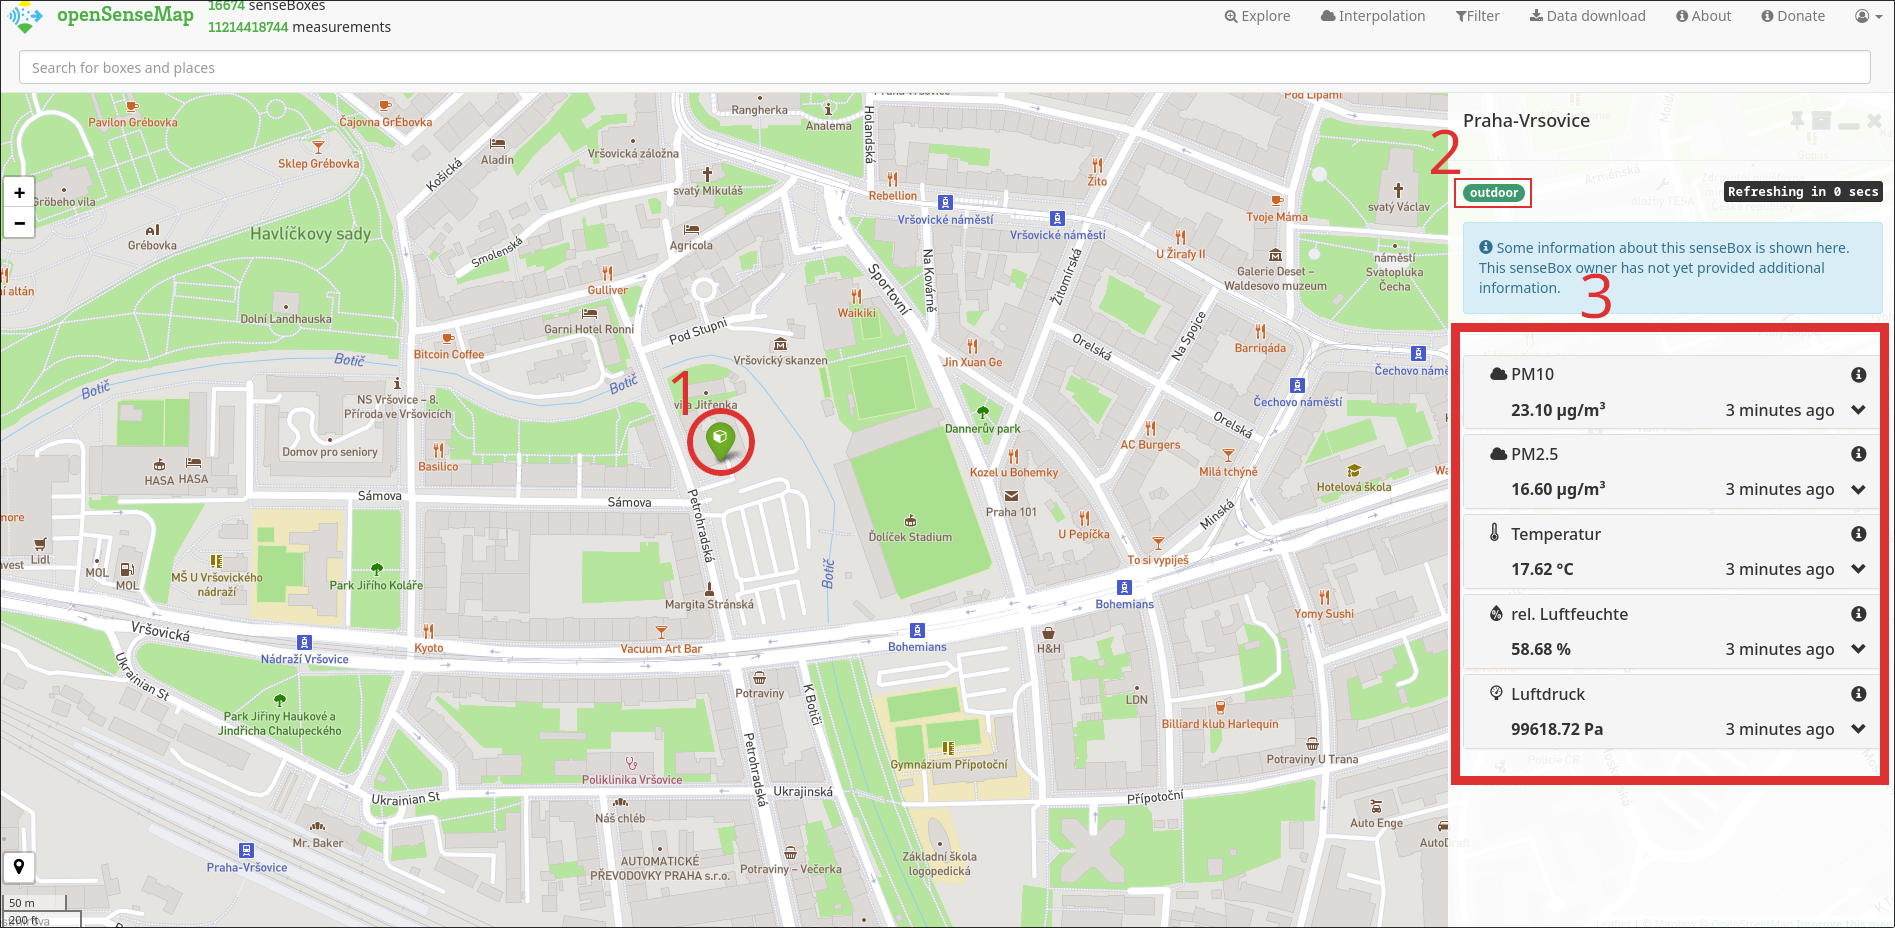
\includegraphics[width=.90\textwidth]{img/opensensemap-map}

\footnotesize \textit{Poznámka:} 1 - konkrétní senzorová stanice zobrazená na mapě, 2 - umístění senzoru (indoor, outdoor, mobile), 3 - měřené veličiny a aktuálně naměřené hodnoty

\footnotesize \textit{Zdroj:} Snímek obrazovky pořízen autorem z webového rozhraní aplikace.
\end{figure}

\begin{figure}[htbp!]\centering
\caption{Bodový graf vybrané měřené veličiny konkrétního senzoru v aplikaci openSenseMap}
\label{obr:opensensemap-sensor-reading}
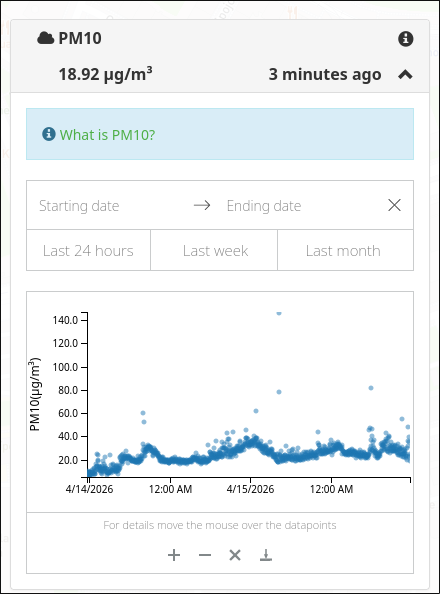
\includegraphics[width=.90\textwidth]{img/opensensemap-reading}

\footnotesize \textit{Poznámka:} Ukázka bodovégo grafu zobrazujícího jednotlivé naměřené hodnoty vybrané veličiny za vybrané časové období pro konkrétní senzor. 

\footnotesize \textit{Zdroj:} Snímek obrazovky pořízen autorem z webového rozhraní aplikace.
\end{figure}

\begin{figure}[htbp!]\centering
\caption{Filtry zobrazení webového rozhraní v aplikaci openSenseMap}
\label{obr:opensensemap-filters}
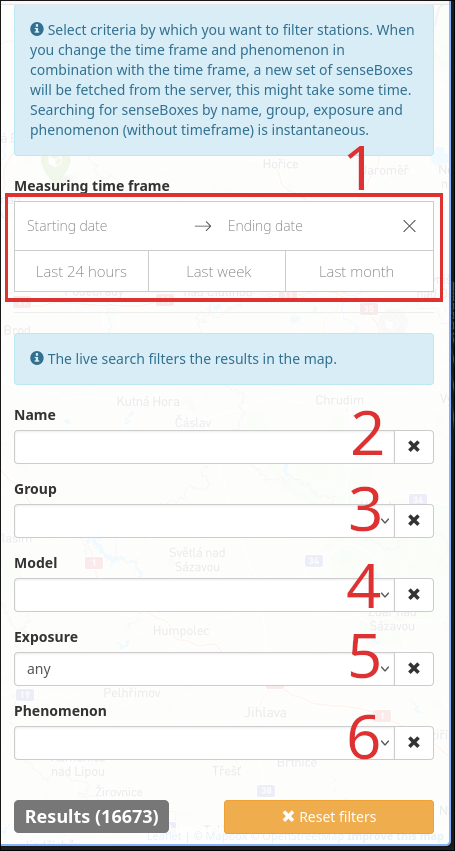
\includegraphics[width=.70\textwidth]{img/opensensemap-filters}

\footnotesize \textit{Poznámka:} 1 - omezení časového období, 2 - omezení dle jména, 3 - omezení dle skupiny, do které uživatel senzor zařadil, 4 - omezení dle modelu (senseBox, Luftdaten, vlastní), 5 - omezení dle typu prostředí (indoor, outdoor, mobile), 6 - omezení dle sledované veličiny

\footnotesize \textit{Zdroj:} Snímek obrazovky pořízen autorem z webového rozhraní aplikace.
\end{figure}


Na rozdíl od aplikací Sensor.Community a OpenAQ nemá platforma openSenseMap pevně daný výčet sledovaných veličin ani předem definovaný seznam podporovaných senzorů. Při registraci senzorové stanice uživatel volně definuje název veličiny, měrnou jednotku a typ senzoru jako textové řetězce. Platforma tak může přijímat data z libovolného senzoru, který uživatel připojí. Pro usnadnění registrace nabízí platforma předdefinované šablony senzorových stanic (např. \textit{senseBox:home} v různých verzích), které obsahují běžné kombinace senzorů pro měření teploty, vlhkosti, atmosférického tlaku, osvětlenosti, UV záření, koncentrace mikročástic PM\textsubscript{2,5} a PM\textsubscript{10}, VOC, CO\textsubscript{2} a hladiny hluku. Tyto šablony jsou však pouze doporučením a uživatel je může libovolně upravit. \parencite{SenseboxOpenSenseMapAPI2026}

Tato otevřenost přináší významnou výhodu ve flexibilitě, neboť platforma není vázána na konkrétní hardware a nevyžaduje aktualizaci při uvedení nového typu senzoru na trh. Zároveň však přináší problémy spojené s konzistencí dat. Stejná fyzikální veličina může být na platformě evidována pod různými názvy (např. \textit{Temperatur}, \textit{Lufttemperatur}, \textit{Temperature}), v různých jednotkách a s různými typy senzorů. Tento stav ztěžuje agregaci a srovnávání dat napříč senzory a vyžaduje od uživatelů dat dodatečnou normalizaci. \parencite{SenseboxOpenSenseMapAPI2026}

Z hlediska veličin relevantních pro IEQ platforma prostřednictvím předdefinovaných šablon podporuje měření teploty vzduchu, relativní vlhkosti, atmosférického tlaku, koncentrace mikročástic (PM\textsubscript{1}, PM\textsubscript{2,5}, PM\textsubscript{4}, PM\textsubscript{10}), VOC (jako odpor senzoru v k$\Omega$), CO\textsubscript{2} (v ppm), osvětlenosti (v lx), UV intenzity (v $\mu$W/cm$^2$), hladiny hluku (v dB(A)) a rychlosti větru. Plynné polutanty jako O\textsubscript{3}, NO\textsubscript{2}, SO\textsubscript{2} a CO nejsou součástí předdefinovaných šablon a v datech platformy se vyskytují pouze ojediněle v rámci uživatelsky definovaných senzorů. \parencite{SenseboxOpenSenseMapAPI2026, OpenSenseMapAPIDocumentation}
